% tRSLguide.tex
% v3.7 released February 2013

\documentclass[]{tRSL2e}

\begin{document}

\jvol{00} \jnum{00} \jyear{2013} \jmonth{February}

\articletype{GUIDE}

\title{{\em{Remote Sensing Letters}} \break \LaTeX\ style guide
for authors (`Own Style')}

\author{A. N. AUTHOR$^{\ast}$$\dag$\thanks{$^\ast$Corresponding
author. Email: latex.helpdesk@tandf.co.uk \vspace{6pt}} and I. T.
CONSULTANT${\ddag}$\\
\vspace{6pt} $\dag$Taylor \& Francis, 4 Park Square, Milton Park,
Abingdon, OX14 4RN, UK\\
$\ddag$ Institut f\"{u}r Informatik, Albert-Ludwigs-Universit\"{a}t,
D-79110 Freiburg, Germany\\
\vspace{6pt}\received{v3.7 released February 2013} }

\maketitle

\begin{abstract}
This guide is for authors who are preparing papers for the Taylor \& Francis journal {\em Remote Sensing Letters} ({\it tRSL}\,) using the \LaTeX\ document preparation system and the class file {\tt
tRSL2e.cls}, which is available via the journal's homepage on the Taylor \& Francis website. Authors planning to submit their papers in \LaTeX\ are advised to use {\tt tRSL2e.cls} as
early as possible in the creation of their files.

\vspace{12pt}\centerline{\bfseries Index to information contained in this guide}\vspace{12pt}

\hbox to \textwidth{\hsize\textwidth\vbox{\hsize18pc
\hspace*{-12pt} {1.}    Introduction\\
\hspace*{7pt} {1.1.}  The {\it tRSL} document class\\
\hspace*{7pt} {1.2.}  Submission of \LaTeX\ articles\\
\hspace*{24pt}        to the journal\\
{2.}    Using the {\it tRSL} class file\\
{3.}    Additional features\\
\hspace*{10pt}{3.1.}  Footnotes to article titles\\
\hspace*{24pt}        and authors' names\\
\hspace*{10pt}{3.2.}  Abstracts\\
\hspace*{10pt}{3.3.}  Lists\\
\hspace*{10pt}{3.4.}  Landscape pages\\
{4.}    Some guidelines for using\\
\hspace*{6pt}        standard features\\
\hspace*{10pt}{4.1.}   Sections\\
\hspace*{10pt}{4.2.}   Illustrations (figures)\\
\hspace*{10pt}{4.3.}   Tables\\
\hspace*{10pt}{4.4.}   Theroem-like environments\\
\noindent \hspace*{7pt} {4.5.}   Typesetting mathematics\\
\hspace*{24pt} {4.5.1.}   Displayed mathematics\\
\hspace*{24pt} {4.5.2.}  Bold math italic symbols\\
\hspace*{24pt} {4.5.3.}   Bold Greek\\
\hspace*{24pt} {4.5.4.}   Upright Greek characters  \\
\hspace*{48pt}            and the upright partial \\
\hspace*{48pt}            derivative sign  \\}
\hspace{-24pt}\vbox{\noindent\hsize18pc
\hspace*{7pt} {4.6.}   Acknowledgements \\
\hspace*{7pt} {4.7.}   Notes \\
\hspace*{7pt} {4.8.}   References \\
\hspace*{24pt} {4.8.1.}   References cited in the\\
\hspace*{48pt}                 text  \\
\hspace*{24pt} {4.8.2.}   The list of references\\
\hspace*{7pt} {4.9.}   Appendices \\
\hspace*{7pt} {4.10.}   {\it tRSL} macros  \\
{5.}    Example of a section heading \\*
\hspace*{7pt}   including {\fontencoding{T1}\scshape{small caps}}, {\it italic}, \\*
\hspace*{7pt}   and bold Greek such as ${\bm\kappa}$ \\
{6.}   {\em tRSL} journal style \\
\hspace*{10pt}{6.1.}   Hyphens, n-rules, m-rules and\\ \hspace*{27pt}minus signs\\
\hspace*{10pt}{6.2.}   References \\
\hspace*{10pt}{6.3.}   Maths fonts\\
\noindent   {7.}   Troubleshooting\\
{8.}   Fixes for coding problems\\
{9.}   Obtaining the tRSL2e class file\\
\hspace*{10pt}{9.1}  Via the Taylor \& Francis \\
\hspace*{24pt}                 website\\
\hspace*{10pt}{9.2}   Via e-mail\\
      }}
\end{abstract}


\section{Introduction}

In order to assist authors in the process of preparing a manuscript for {\itshape Remote Sensing Letters} ({\it tRSL}), the journal's layout style has been implemented as a \LaTeXe\ class file based on the {\tt article} document class. A \textsc{Bib}\TeX\ style file is also provided to assist with the formatting of your references in a style appropriate to that of the journal.

Commands that differ from or are provided in addition to the standard \LaTeXe\ interface are explained in this guide. The guide alone is not intended as a substitute for an appropriate \LaTeXe\ manual.

The \texttt{tRSLguide.tex} file can also be used as a template for composing an article for submission by cutting, pasting, inserting and
deleting text as appropriate, using the \LaTeX\ environments provided (e.g. \verb"\begin{equation}",
\verb"\begin{enumerate}").

{\bf{Please note that the index following the abstract in this guide is provided for information only. An index is not required in submitted papers.}}


\subsection{The {\bi tRSL} document class}

The \textit{tRSL} class file preserves the standard \LaTeXe\ interface such that any document that can
be produced using {\tt article.cls} can also be produced using the {\it tRSL} document class.
However, the measure (the width of the text on a page) is narrower than the default for {\tt article.cls}, therefore line breaks
will change and some long equations may need to be reformatted accordingly.

If your article is accepted for publication in the journal, it will be typeset in Monotype Times. As most authors do not own this font, it is likely that the page make-up will alter with the change of font. For this reason, please ignore details such as slightly long lines of text, page stretching, or figures falling out of synchronization with their citations in the text: these details will be dealt with by the typesetter. Similarly, it is unnecessary to spend time addressing warnings in the log file -- if your .tex file compiles to produce a PDF file that correctly reflects how you wish your paper to appear when printed, such warnings will not prevent your source files being imported into the typesetter's program.


\subsection{Submission of \LaTeX\ articles to the journal}\label{S1.2}

Manuscripts for possible publication in the journal should be submitted to the Editors for review as directed in the journal's Instructions for Authors, which may be found at {\tt{http://www.tandf.co.uk/journals/authors/trslauth.asp}}.

Manuscripts created using \LaTeX\ should be converted to PDF format prior to submission. The \LaTeX\ source files and any graphics files will be required in addition to the final PDF version when final, revised versions of accepted manuscripts are submitted.

`Open-source' \LaTeXe\ should be used in preference to proprietary systems such as TCILaTeX or Scientific WorkPlace; similarly, class files such as REVTeX4 that produce a document in the style of a different publisher and journal should not be used for preference.

Authors who wish to incorporate Encapsulated PostScript artwork directly in their articles can do so by using
Tomas Rokicki's {\tt EPSF} macros (which are supplied with the DVIPS PostScript driver). See Section~\ref{eps},
which also demonstrates how to treat landscape pages. Please remember to supply any additional figure macros you
use with your article in the preamble before \verb"begin{document}". Authors should not attempt to use
implementation-specific \verb"\special"s directly.

Ensure that any author-defined macros are gathered together in the source file, just before the
\verb"\begin{document}" command.

Please note that, if serious problems are encountered with the coding of a paper (missing author-defined macros,
for example), it may prove necessary to divert the paper to conventional typesetting, i.e. it will be re-keyed.


\section{Using the {\bi tRSL} class file}

If the file {\tt tRSL2e.cls} is not already in the appropriate system directory for \LaTeXe\ files, either
arrange for it to be put there, or copy it to your working folder. In order to use the {\it tRSL} document class, replace
the command \verb"\documentclass{article}" at the beginning of your document with the command \verb"\documentclass{tRSL2e}".

The following document-class options should {\em not\/} be used with the {\it tRSL} class file:
%
\begin{itemize}
   \item {\tt 10pt}, {\tt 11pt}, {\tt 12pt} -- unavailable;
   \item {\tt oneside}, {\tt twoside} -- not necessary, oneside is the default;
   \item {\tt leqno} and {\tt titlepage} -- should not be used;
   \item {\tt onecolumn} -- not necessary as it is the default style.
\end{itemize}
%
The {\tt geometry} package and commands associated with it should also not be used to adjust the page dimensions.


\section{Additional features}

\subsection{Footnotes to article titles and authors' names}

The \verb"\thanks" control sequence may be used to produce a footnote to either the title or authors' names.
Footnote symbols for this purpose should be used in the order: $\dagger$ (coded as \verb"\dagger"), $\ddagger$ (\verb"\ddagger"), $\S$ (\verb"\S"), $\P$ (\verb"\P"), $\|$ (\verb"\|"),\break
$\dagger\dagger$ (\verb"\dagger\dagger"), $\ddagger\ddagger$ (\verb"\ddagger\ddagger"), $\S\S$ (\verb"\S\S"), $\P\P$ (\verb"\P\P"), $\|\|$ (\verb"\|\|").

Footnotes to the main text will automatically be assigned the superscript
 symbols 1, 2, 3,... by the class file, beginning afresh on each
page.\footnote{These symbols will be changed to the style of the journal by the
 typesetter during preparation of your proofs. If preferred, the \texttt{endnotes} package
 may be used instead to set the notes in consecutive order at the end
 of your text, before the bibliography.}

The title, author(s) and affiliation(s) should be followed by the {\verb"\maketitle"} command. If preparing an anonymized version for peer review, {\verb"\maketitle"} may follow directly after the title in order to shield the authors' identities from the reviewers.


\subsection{Abstracts}

At the beginning of your article, the title should be generated in the usual way using the {\verb"\maketitle"}
command. Immediately following the title you should include an abstract. The abstract should be enclosed within
an {\tt abstract} environment. For example, the titles for this guide were produced by the following source code:
%
\begin{verbatim}
\title{{\itshape Remote Sensing Letters}\break
\LaTeX\ style guide for authors (`Own Style')}

\author{A. N. AUTHOR$^{\ast}$$\dag$\thanks{$^\ast$Corresponding
author. Email: latex.helpdesk@tandf.co.uk \vspace{6pt}} and I. T.
CONSULTANT${\ddag}$\\
\vspace{6pt} $\dag$Taylor \& Francis, 4 Park Square, Milton Park,
Abingdon, OX14 4RN, UK\\
$\ddag$ Institut f\"{u}r Informatik, Albert-Ludwigs-Universit\"{a}t,
D-79110 Freiburg, Germany\\
\vspace{6pt}\received{v3.7 released February 2013} }

\maketitle

\begin{abstract}
This guide is for authors who are preparing papers for the Taylor
\& Francis journal {\em Remote Sensing Letters} ({\it tRSL}\,)
using the \LaTeX\ document preparation system and the class file
{\tt tRSL2e.cls}, which is available via the journal's homepage on
the Taylor \& Francis website. Authors planning to submit papers in
\LaTeX\ are advised to use {\tt tRSL2e.cls} as early as possible in
the creation of their files.
\end{abstract}
\end{verbatim}


\subsection{Lists}

The {\it tRSL} style provides numbered and unnumbered lists using the {\tt enumerate} environment and bulleted
lists  using the {\tt itemize} environment.

The enumerated list numbers each list item with roman numerals by default, for example:
%
\begin{enumerate}
   \item first item
   \item second item
   \item third item
\end{enumerate}
%
Alternative numbering styles can be achieved by inserting an optional argument in square brackets after the
\verb"\item". For example, the list
%
\begin{enumerate}
   \item[(1)] first item
   \item[(2)] second item
   \item[(3)] etc. \ldots
\end{enumerate}
%
was produced by:
%
\begin{verbatim}
\begin{enumerate}
   \item[(1)] first item
   \item[(2)] second item
   \item[(3)] etc. \ldots
\end{enumerate}
\end{verbatim}
%
Unnumbered lists are also provided using the {\tt enumerate} environment. For example,
\begin{enumerate}
   \item[] First unnumbered item which has no label and is indented from
         the left margin.
   \item[] Second unnumbered item.
   \item[] Third unnumbered item.
\end{enumerate}
was produced by:
%
\begin{verbatim}
\begin{enumerate}
  \item[] First unnumbered item...
  \item[] Second unnumbered item.
  \item[] Third unnumbered item.
\end{enumerate}
\end{verbatim}
%
Bulleted lists are provided using the {\tt itemize} environment. For example,
\begin{itemize}
\item First bulleted item
\item Second bulleted item
\item Third bulleted item
\end{itemize}
was produced by:
\begin{verbatim}
  \begin{itemize}
  \item First bulleted item
  \item Second bulleted item
  \item Third bulleted item
  \end{itemize}
\end{verbatim}


\subsection{Landscape pages}\label{eps}

If a table or illustration is too wide to fit the standard measure, it must be turned, with its caption, through
90$^{\circ}$ anticlockwise. Landscape illustrations and/or tables can be produced directly using the tRSL2e class
file using \verb"\usepackage{rotating}" after \verb"\documentclass{tRSL2e}". The following commands can be used
to produce such pages.
%
\begin{verbatim}
\setcounter{figure}{2}
\begin{sidewaysfigure}
\centerline{\epsfbox{fig1.eps}}
\caption{This is an example of a figure caption.}
\label{landfig}
\end{sidewaysfigure}
\end{verbatim}
%
\begin{verbatim}
\setcounter{table}{0}
\begin{sidewaystable}
  \tbl{The Largest Optical Telescopes.}
    \begin{tabular}{@{}llllcll}
    .
    .
    .
  \end{tabular}\label{tab1}
\end{sidewaystable}
\end{verbatim}
%
Before any float environment, use the \verb"\setcounter" command
as above to fix the numbering of the caption. Subsequent captions
will then be automatically renumbered accordingly.


\section[]{Some guidelines for using standard features}

The following notes may help you achieve the best effects with the tRSL2e Class file.

\subsection{Sections}

\LaTeXe\ provides five levels of section headings and they are all defined in the tRSL2e Class file:
\begin{enumerate}
   \item \verb"\section"
   \item \verb"\subsection"
   \item \verb"\subsubsection"
   \item \verb"\paragraph"
   \item \verb"\subparagraph"
\end{enumerate}
Numbering is automatically generated for section, subsection, subsubsection and paragraph headings.  If you need
additional text styles in the headings, see the examples in Section~5.


\subsection{Illustrations (figures)}

The {\it tRSL} class file will cope with most positioning of your illustrations and you should not normally use the optional positional qualifiers of the {\tt figure} environment, which would override these decisions. See `Instructions for Authors' in the journal's homepage on the Taylor \& Francis website for how to submit artwork (please note that requests to supply figures separately from text are addressed to authors using Microsoft Word; authors using \LaTeX\ may include illustrations at the appropriate locations in their PDF file). The original source files of any illustrations will be required when the final, revised version is submitted. Authors should ensure that their figures are suitable (in terms of lettering size, etc.) for the reductions they intend.

Figure captions should be below the figure itself, therefore the \verb"\caption" command should appear after the
figure. For example, figure~\ref{sample-figure} with caption and sub-captions is produced using the following
commands:
%
\begin{verbatim}
\begin{figure}
\begin{center}
\subfigure[An example of an individual figure sub-caption.]{
\resizebox*{5cm}{!}{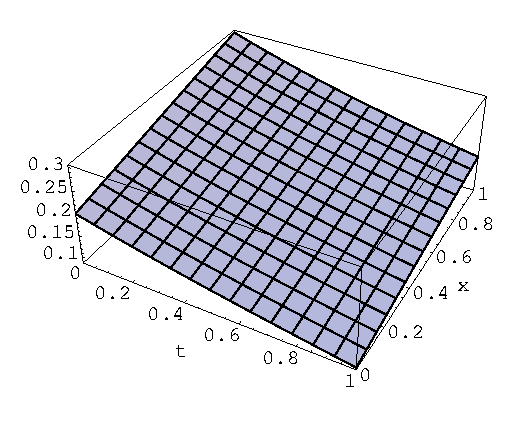
\includegraphics{senu_gr1.eps}}}\hspace{5pt}
\subfigure[An example of an individual figure sub-caption.]{
\resizebox*{5cm}{!}{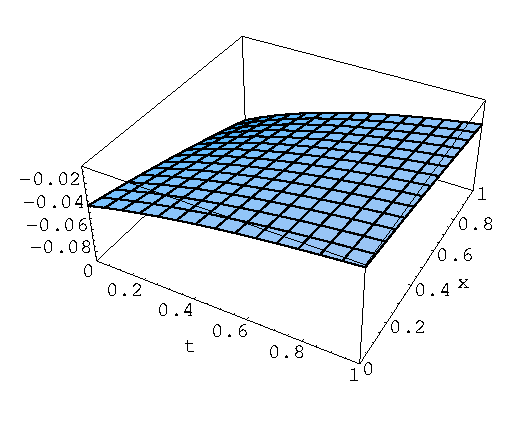
\includegraphics{senu_gr2.eps}}}
\caption{\label{fig2} Example of a two-part figure with individual
sub-captions showing that captions are flush left and justified if
greater than one line of text, otherwise centred under the figure.}
\label{sample-figure}
\end{center}
\end{figure}
\end{verbatim}

\begin{figure}
\begin{center}
\subfigure[An example of an individual figure sub-caption.]{
\resizebox*{5cm}{!}{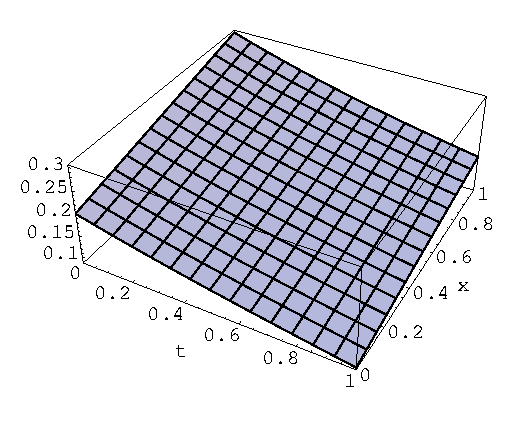
\includegraphics{senu_gr1.eps}}}\hspace{5pt}
\subfigure[An example of an individual figure sub-caption.]{
\resizebox*{5cm}{!}{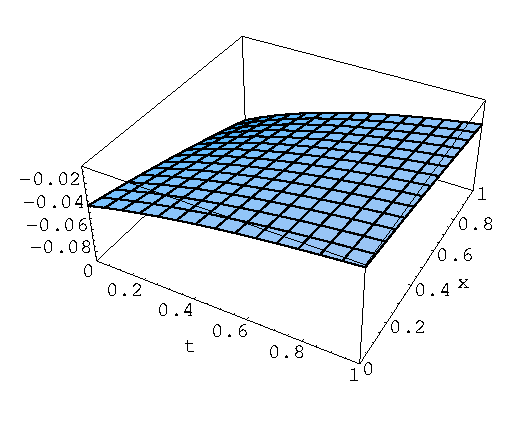
\includegraphics{senu_gr2.eps}}}
\caption{\label{fig2} Example of a two-part figure with individual
sub-captions showing that captions are flush left and justified if
greater than one line of text, otherwise centred under the figure.}
\label{sample-figure}
\end{center}
\end{figure}

To ensure that figures are correctly numbered automatically, the \verb"\label{}" command should be inserted just
after \verb"\caption{}".


\subsection{Tables}

The {\it tRSL} class file will cope with most positioning of your tables and you should not normally use the optional
positional qualifiers of the {\tt table} environment, which would override these decisions. The table caption
appears above the body of the table in {\it tRSL} style, therefore the \verb"\tbl" command should appear before
the body of the table.

The {\tt tabular} environment can be used as illustrated here to produce tables with single thick and thin horizontal rules, which
are allowed, if desired. Thick rules should be used at the head and foot only and thin rules elsewhere.

Commands to redefine quantities such as \verb"\arraystretch" should be omitted. For example, table~\ref{symbols}
is produced using the following commands. Note that \verb"\rm" will produce a roman character in math mode. There
are also \verb"\bf" and \verb"\it", which produce bold face and text italic in math mode.

\begin{table}
  \tbl{Radio-band beaming model parameters for\\ {FSRQs and BL Lacs.}}
{\begin{tabular}[l]{@{}lcccccc}
\toprule
  Class$^{\rm a}$ & $\gamma _1$ & $\gamma _2$$^{\rm b}$
         & $\langle \gamma \rangle$
         & $G$ & $|{\bm f}|$ & $\theta _{c}$ \\
\colrule
  BL Lacs &5 & 36 & 7 & $-4.0$
         & $1.0\times 10^{-2}$ & 10$^\circ$ \\
  FSRQs & 5 & 40 & 11 & $-2.3$
         & $0.5\times 10^{-2}$ & 14$^\circ$ \\
\botrule
\end{tabular}}
\tabnote{$^{\rm a}$This footnote shows what footnote symbols to use.}
\tabnote{$^{\rm b}$This footnote shows the text turning over when a long footnote is added.}
\label{symbols}
\end{table}


\begin{verbatim}
\begin{table}
  \tbl{Radio-band beaming model parameters for {FSRQs and BL Lacs.}}
{\begin{tabular}{@{}lcccccc}
\toprule
  Class$^{\rm a}$ & $\gamma _1$ & $\gamma _2$$^{\rm b}$
         & $\langle \gamma \rangle$
         & $G$ & $|{\bm f}|$ & $\theta _{c}$ \\
\colrule
  BL Lacs &5 & 36 & 7 & $-4.0$
         & $1.0\times 10^{-2}$ & 10$^\circ$ \\
  FSRQs & 5 & 40 & 11 & $-2.3$
         & $0.5\times 10^{-2}$ & 14$^\circ$ \\
\botrule
\end{tabular}}
\tabnote{$^{\rm a}$This footnote shows what footnote symbols to use.}
\tabnote{$^{\rm b}$This footnote shows the text turning over when a
 long footnote is added.}
\label{symbols}
\end{table}
\end{verbatim}

To ensure that tables are correctly numbered automatically, the \verb"\label{}" command should be inserted just before
\verb"\end{table}". 

Tables produced using the {\tt booktabs} package of macros for typesetting tables are also compatible with the {\it tRSL} class file.


\subsection{Theorem-like environments}

A predefined \verb"proof" environment is provided by the \verb"amsthm" package (which is called by the class file), as follows:

\begin{proof}
More recent algorithms for solving the semidefinite programming relaxation
are particularly efficient, because they explore the structure of the
MAX-CUT problem.
\end{proof}
\noindent This was produced by simply typing:
%
\begin{verbatim}
\begin{proof}
More recent algorithms for solving the semidefinite programming
relaxation are particularly efficient, because they explore the
structure of the MAX-CUT problem.
\end{proof}
\end{verbatim}
%
Other theorem-like environments (theorem, lemma, corollary, etc.) in your document need to be defined as required, e.g. using \verb"\newtheorem{theorem}{Theorem}" in the preamble of your .tex file before \verb"begin{document}". The format of the text in these environments will be changed if necessary to match the style of the journal by the typesetter during preparation of your proofs.


\subsection{Typesetting mathematics}\label{TMth}

\subsubsection{Displayed mathematics}

The {\it tRSL} class file will set displayed mathematics centred on the measure without equation numbers, provided
that you use the \LaTeXe\ standard control sequences open (\verb"\[") and close (\verb"\]") square brackets as
delimiters. The equation
\[
  \sum_{i=1}^p \lambda_i = {\rm trace}({\textrm{\bf S}})\qquad
  i\in {\mathbb R}
\]
\normalfont was typeset using the commands
%
\begin{verbatim}
\[
  \sum_{i=1}^p \lambda_i = {\rm trace}({\textrm{\bf S}})\qquad
  i\in {\mathbb R}
\].
\end{verbatim}

For those of your equations that you wish to be automatically
numbered sequentially throughout the text, use the {\tt{equation}}
environment, e.g.

\begin{equation}
  \sum_{i=1}^p \lambda_i = {\rm trace}({\textrm{\bf S}})\qquad
  i\in {\mathbb R}
\end{equation}
%
was typeset using the commands

\begin{verbatim}
\begin{equation}
  \sum_{i=1}^p \lambda_i = {\rm trace}({\textrm{\bf S}})quad
  i\in {\mathbb R}
\end{equation}
\end{verbatim}

Part numbers for sets of equations may be generated using the
{\tt{subequations}} environment, e.g.
\begin{subequations} \label{subeqnexample}
\begin{equation}
        \varepsilon \rho w_{tt}(s,t)
        =
        N[w_{s}(s,t),w_{st}(s,t)]_{s},
        \label{subeqnpart}
\end{equation}
\begin{equation}
        w_{tt}(1,t)+N[w_{s}(1,t),w_{st}(1,t)] = 0,
\end{equation}
\end{subequations}
which was generated using the control sequences

\begin{verbatim}
\begin{subequations} \label{subeqnexample}
\begin{equation}
        \varepsilon \rho w_{tt}(s,t)
        =
        N[w_{s}(s,t),w_{st}(s,t)]_{s},
        \label{subeqnpart}
\end{equation}
\begin{equation}
        w_{tt}(1,t)+N[w_{s}(1,t),w_{st}(1,t)] = 0,
\end{equation}
\end{subequations}
\end{verbatim}
This is made possible by the package {\tt{subeqn}}, which is called
by the class file. If you put the \verb"\label{}" just after the
\verb"\begin{subequations}" line, references will be to the
collection of equations, `(\ref{subeqnexample})' in the example
above. Or, like the example code above, you can reference each
equation individually -- e.g. `(\ref{subeqnpart})'.


\subsubsection{Bold math italic symbols}

To get bold math italic you can use \verb"\bm", which works for
all sizes, e.g.
%
\begin{verbatim}
\sffamily
\begin{equation}
   {\rm d}({\bm s_{t_{\bm u}}) = \langle{\bm\alpha({\sf{\textbf L}})}
   [RM({\bm X}_y + {\bm s}_t) - RM({\bm x}_y)]^2 \rangle
\end{equation}
\normalfont
\end{verbatim}
%
produces\sffamily
\begin{equation}
   {\rm d}({\bm s_{t_{\bm u}}}) = \langle {\bm\alpha({\sf{\textbf L}})}[RM({\bm X}_y
   + {\bm s}_t) - RM({\bm x}_y)]^2 \rangle
\end{equation}\normalfont
Note that subscript, superscript, subscript to subscript, etc.
sizes will take care of themselves and are italic, not bold,
unless coded individually. \verb"\bm" produces the same effect as
\verb"\boldmath". \verb"\sffamily"...\verb"\normalfont" allows
upright sans serif fonts to be created in math mode by using the
control sequence `\verb"\sf"'.


\subsubsection{Bold Greek}\label{boldgreek}

Bold lowercase as well as uppercase Greek characters can be obtained by \verb"{\bm \gamma}", which gives ${\bm
\gamma}$, and \verb"{\bm \Gamma}", which gives ${\bm \Gamma}$.


\subsubsection{Upright lowercase Greek characters and the upright partial derivative sign}\label{upgreek}

Upright lowercase Greek characters can be obtained with the Class file by inserting the letter `u' in the
control code for the character, e.g. \verb"\umu" and \verb"\upi" produce $\umu$ (used, for example, in the
symbol for the unit microns -- $\umu{\rm m}$) and $\upi$ (the ratio of the circumference to the diameter of a
circle). Similarly, the control code for the upright partial derivative $\upartial$ is \verb"\upartial".


\subsection{Acknowledgements}

This unnumbered section, e.g. \verb"\section*{Acknowledgement(s)}", should be used for thanks, grant details, etc.
and placed before any Notes or References sections.


\subsection{Notes}

This unnumbered section, e.g. \verb"\section*{Note(s)}", may be placed before any References section.


\subsection{References}\label{refs}

\subsubsection{References cited in the text} References should be cited in the text in
author--date (Harvard) style -- e.g. `(Smith 1985, Jones 1986, Trevor {\itshape{et al.}} 1987, Bloggs
{\itshape{et al.}} 2001)' or `... see Smith (1985) ...' (note that these references have been cited in
chronological order and `{\itshape{et al.}}' has been used for two or more authors)'. References should be
listed in the references list at the end of the main text in alphabetical order, then chronologically, with no
issue numbers and full page ranges where appropriate. A smaller font than in the main body text should be used,
with a hanging indent. Each bibliographical entry has a key, which is assigned by the author and used to refer
to that entry in the text. In this document, the key \verb"ed84" in the citation form \verb"\citep{ed84}"
produces `\citep{ed84}', and the keys \verb"ed84", \verb"aiex02", \verb"glov00" and \verb"mtw73" in the citation
form \verb"\citep{ed84,aiex02,glov00,mtw73}" produce `\citep{ed84,aiex02,glov00,mtw73}'. The appropriate
citation style in the text for different situations can be produced by \verb"\citet{aiex00}" for
`\citet{aiex00}', \verb"\citealt{lam86}" for `\citealt{lam86}' and \verb"\citet{aiex00,aiex02,hk96,fzf88}" for
`\citet{aiex00,aiex02,hk96,fzf88}'. Optional notes may be included at the beginning and end of a citation by the
use of square brackets, e.g. \verb"\citep[see][and" \verb"references" \verb"therein]{aiex02}" produces
`\citep[see][and references therein]{aiex02}'. Citation of the year alone may be produced by
\verb"\citeyear{neu83}", i.e. `\citeyear{neu83}', or \verb"\citeyearpar{neu83}", i.e. `\citeyearpar{neu83}'.

\subsubsection{The list of references}

The following list shows some references prepared in the style of the journal:
%
\begin{thebibliography}{9}

\bibitem[\protect\citeauthoryear{Aiex {\itshape{et~al.}}}{2000}]{aiex00}
\textsc{Aiex, R.M., Resende, M.G.C., Pardalos, P.M. {\normalfont and} Toraldo,
  G.}, 2000, GRASP with path-relinking for the three-index assignment problem.
  Technical report, AT\&T Labs-Research.

\bibitem[\protect\citeauthoryear{Aiex {\itshape{et al.}}}{2002}]{aiex02}
A{\sc iex}, R.M., R{\sc esende},  M.G.C. and R{\sc ibeiro}, C.C.,
2002, Probability distribution of solution time in GRASP: an
experimental investigation. Available online at:
www.graspintime.com (accessed 23 October 2003).

\bibitem[\protect\citeauthoryear{Edwards {\itshape{et~al.}}}{1984}]{ed84}
\textsc{Edwards, D.M.F., Madden, P.A. {\normalfont and} McDonald, I.R.}, 1984,
Nanotechnology in fibrous materials -- a new perspective. {\itshape Textile Progress}, \textbf{51}, pp. 1141--1151.

\bibitem[\protect\citeauthoryear{French}{1988}]{fzf88}
\textsc{French, F.}, 1988, English title of a chapter in the translation of a
  book in a foreign language. In     {\itshape Title of a Book in Another Language
  (Quoted in that Language)}, {P.} Smith (Transl.)   (New York: Dover)
  (original work published 1923).

\bibitem[\protect\citeauthoryear{Glover}{2000}]{glov00}
\textsc{Glover, F.}, 2000, Multi-start and strategic oscillation
  methods -- principles to exploit adaptive memory. In {\itshape Computing Tools
  for Modeling, Optimization and Simulation: Interfaces in Computer Science and
  Operations Research} (2nd  edn), M.~Laguna {\normalfont and} J.L.
  Gonz\'{a}les-Velarde (Eds), pp. 1--24  (Boston, MA: Kluwer Academic).

\bibitem[\protect\citeauthoryear{Kern}{1997}]{hk96}
\textsc{Kern, H.}, 1997, The resurgent Japanese economy and a Japan--United
  States free trade agreement. In {\itshape Proceedings of the }{\itshape 4th
  International Conference on the Restructuring of the Economic and Political
  System in Japan and Europe}, 21--25 May 1996, Milan, Italy (Singapore: World
  Scientific), pp. 147--156.

\bibitem[\protect\citeauthoryear{Lamport}{1996}]{lam86}
L{\sc amport}, L., 1986, Efficient algorithms for layer assignment
problems. PhD thesis, University of Princeton, NJ.

\bibitem[\protect\citeauthoryear{Misner}{1973}]{mtw73}
\textsc{Misner, C.W.} (Ed.), 1973, Efficient algorithms for layer assignment
  problems. In {\itshape Gravitation} (2nd  edn), Einstein's Legacy Vol. 5, pp. 231--256
  (San Francisco, CA: Freeman).

\bibitem[\protect\citeauthoryear{Neumann}{1983}]{neu83}
\textsc{Neumann, M.}, 1983, Parallel GRASP with path-relinking for job
  shop scheduling. {\itshape International Journal of Geographical Information
  Science}, \textbf{50}, pp. 841--843.

\end{thebibliography}
\bigskip
\noindent This was produced by typing:
\medskip
\begin{verbatim}
\bibitem[\protect\citeauthoryear{Aiex {\itshape{et~al.}}}{2000}]{aiex00}
\textsc{Aiex, R.M., Resende, M.G.C., Pardalos, P.M. {\normalfont and}
 Toraldo, G.}, 2000, GRASP with path-relinking for the three-index
 assignment problem. Technical report, AT\&T Labs-Research.

\bibitem[\protect\citeauthoryear{Aiex {\itshape{et al.}}}{2002}]{aiex02}
A{\sc iex}, R.M., R{\sc esende},  M.G.C. and R{\sc ibeiro}, C.C.,
 2002, Probability distribution of solution time in GRASP: an
 experimental investigation. Available online at:
 www.graspintime.com (accessed 23 October 2003).

\bibitem[\protect\citeauthoryear{Edwards {\itshape{et~al.}}}{1984}]{ed84}
\textsc{Edwards, D.M.F., Madden, P.A. {\normalfont and} McDonald, I.R.},
 1984, Nanotechnology in fibrous materials -- a new perspective.
 {\itshape Textile Progress}, \textbf{51}, pp. 1141--1151.

\bibitem[\protect\citeauthoryear{French}{1988}]{fzf88}
\textsc{French, F.}, 1988, English title of a chapter in the translation
 of a book in a foreign language. In {\itshape Title of a Book in
 Another Language (Quoted in that Language)}, {P.} Smith (Transl.)
 (New York: Dover) (original work published 1923).

\bibitem[\protect\citeauthoryear{Glover}{2000}]{glov00}
\textsc{Glover, F.}, 2000, Multi-start and strategic oscillation
 methods -- principles to exploit adaptive memory. In {\itshape
 Computing Tools for Modeling, Optimization and Simulation: Interfaces
 in Computer Science and Operations Research} (2nd  edn), M.~Laguna
 {\normalfont and} J.L. Gonz\'{a}les-Velarde (Eds), pp. 1--24 (Boston,
 MA: Kluwer Academic).

\bibitem[\protect\citeauthoryear{Kern}{1997}]{hk96}
\textsc{Kern, H.}, 1997, The resurgent Japanese economy and a
 Japan--United States free trade agreement. In {\itshape Proceedings of
 the 4th International Conference on the Restructuring of the Economic
 and Political System in Japan and Europe}, 21--25 May 1996, Milan,
 Italy (Singapore: World Scientific), pp. 147--156.

\bibitem[\protect\citeauthoryear{Lamport}{1996}]{lam86}
L{\sc amport}, L., 1986, Efficient algorithms for layer assignment
 problems. PhD thesis, University of Princeton, NJ.

\bibitem[\protect\citeauthoryear{Misner}{1973}]{mtw73}
\textsc{Misner, C.W.} (Ed.), 1973, Efficient algorithms for layer
 assignment problems. In {\itshape Gravitation} (2nd  edn), Einstein's
 Legacy Vol. 5, pp. 231--256 (San Francisco, CA: Freeman).

\bibitem[\protect\citeauthoryear{Neumann}{1983}]{neu83}
\textsc{Neumann, M.}, 1983, Parallel GRASP with path-relinking for job
 shop scheduling. {\itshape International Journal of Geographical
 Information Science}, \textbf{50}, pp. 841--843.
\end{verbatim}

\medskip
\noindent Each entry takes the form:
\medskip
\begin{verbatim}
\bibitem{key} Bibliography entry
\end{verbatim}

\noindent where `{\tt key}' is the tag that is to be used as an argument for the \verb"\cite{}" command in the text of the article and `{\tt Bibliography entry}' is the material that is to appear in the list of references, suitably formatted.

Instead of typing the bibliography by hand, you may prefer to create the list of references using a B{\sc ib}\TeX\ database. Include the lines \vspace{12pt}

\noindent\verb"\bibliographystyle{tRSL}"
\newline\verb"\bibliography{tRSLguide}"
\vspace{12pt}

\noindent where the list of references should appear, where tRSL.bst is the B{\sc ib}\TeX\ style file for this journal and tRSLguide.bib is the database of bibliographic details for the references section included with the {\itshape tRSL} \LaTeX\ style package (to be replaced with the name of your own B{\sc ib}\TeX\ database). The \LaTeXe\ source file of your paper will extract from your .bib file only those references that are cited in that paper and list them in the References section of it.

Please ensure you include either a copy of your .bib file or the final generated .bbl file among your source files if your .tex file does not contain a hand-typed bibliography.

\subsection{Appendices}

Appendices should be set after the references, beginning with the command \verb"\appendices" followed by the
command \verb"\section" for each appendix title, e.g.
%
\begin{verbatim}
\appendices
\section{This is the title of the first appendix}
\section{This is the title of the second appendix}
\end{verbatim}

\noindent produces\medskip

\noindent Appendix A: This is the title of the first appendix

\noindent Appendix B: This is the title of the second appendix

\medskip
Subsections, equations, figures, tables, etc. within
appendices will then be automatically numbered as appropriate.

\subsection{{\bi tRSL} macros}

Table~\ref{macros} gives a list of macros for use with {\it tRSL}. The list displays each macro's code and a
description/demonstration of its function.

\begin{table} \tbl{{\it tRSL} macros.}{\begin{tabular}{@{}ll}
\toprule
$\backslash$thanks\{title-page footnote to article title & e.g. `Corresponding author. E-mail:\\
or author\} & A.N. Author@uiowa.edu'\\\cr
$\backslash$begin\{abstract\}...$\backslash$end\{abstract\} & for abstract on titlepage\\\\ $\backslash$bm\{math
and symbols\} & bold italic $\bm{math\;and\;symbols}$\\\cr $\backslash$bi\{text\} & bold italic \bi{text}\\\cr
$\backslash$sf\{text or upright symbols in math mode\} & sans serif \sf{text} or
$\sf{upright\;symbols\;in\;math\;mode}$\\
\botrule
\end{tabular}}
\label{macros}
\end{table}

\section{Example of a section heading including
   {\fontencoding{T1}\scshape{small caps}}, {\bi italic},
   and bold Greek such as ${\bm\kappa}$}\label{headings}

%
The following code shows how to achieve this section head:
%
\begin{verbatim}
\section{Example of a section heading including
   {\fontencoding{T1}\scshape{small caps}}, {\bi italic},
   and bold Greek such as ${\bm\kappa}$}\label{headings}
\end{verbatim}
%
%%%%%%%%%%%%%%%%%%%%%%%%%%%%%%%%%%%%
%

\section{{\textit{tRSL}} journal style}

The notes given here relate to common style errors found in  {{\it tRSL}} manuscripts, but are {\itshape not\/}
intended to be exhaustive.

\subsection{Hyphens, N-rules, M-rules and minus signs}\label{dashes}

\begin{enumerate}
\item[(i)] Hyphens (one dash in TeX/\LaTeXe). Hyphenation should be used sparingly in {\it tRSL}. Generally, prefixes usually require hyphens: pre-, mid- (e.g. mid-1960s, pre-1978).
\item[(ii)] N-rules (also called en-rules or n-rules)(two dashes in \TeX/\LaTeXe). Spaced N-rules ( -- ) are used for parenthetical dashes, that is, to extract a part of a sentence: `The idea -- and it was her idea -- was exciting.' Otherwise, unspaced N-rules (--) are used when the first part of a compound does not modify the second, and are used in place of `and' or `to', for example, the `research--practitioner interface'; `red--green shift'; the `period 1920--1930'.
\item[(iii)] M-rules (also called em-rules or m-rules)(three dashes in \TeX/\LaTeXe). Unspaced M-rules (---) are only used to indicate the omission of a name, part of a name, or a date, for example, `Mr S--- entered the class.'
\item[(iv)] The minus sign (one dash in \TeX/\LaTeXe) is produced
automatically in math mode by use of a single dash, e.g.
\begin{equation}
y_{i} \in \{-1, 1 \} \quad \forall i \in V
\end{equation}
\noindent where $|-V|=A^2+B^2$\medskip

\noindent is produced by

\begin{verbatim}
\begin{equation}
y_{i} \in \{-1, 1 \} \quad \forall i \in V
\end{equation}
\noindent where $|-V|=A^2+B^2$
\end{verbatim}

\end{enumerate}


\subsection{References}

It is important to use the correct reference style, details  of which can be found in Section~\ref{refs} above.

\subsection{Maths fonts}
Scalar  variables should be mediumface italic (e.g. $s$ for speed); vectors should be bold italic (e.g. $\bm v$
for velocity); matrices should be bold roman (upright) (e.g. $\bf A$), and tensors should be bold upright sans
serif (e.g. {\sffamily{\textbf L}}). Differential d, partial differential $\upartial$, complex i, exponential e,
superscript T for `transpose', sin, cos, tan, log, etc., should all be roman. Openface, or `blackboard', fonts
can be used, for example, for the integers $\mathbb Z$ and the reals $\mathbb R$. Sub/superscripts that are
physical variables should be italic, while those  that are labels should be roman (e.g.\ $C_p$, $T_{\rm eff}$).
Displayed equations should have end-of-line punctuation appropriate to the running text sentence of which they
form a part.


\section{Troubleshooting}

Authors may from time to time encounter problems with the  preparation
of their papers in \LaTeX. The appropriate  action  to
take will depend on the nature of the problem -- the following is
intended to act as a guide.
%
\begin{enumerate}
\item If the problem is with \LaTeX\ itself, rather than with the
actual macros, please refer to the appropriate handbooks for
initial advice.\footnote{\TeX: Knuth, D., 1986, {\it The \TeX\
book} (New York: Addison--Wesley); \LaTeXe: Lamport, L., 1994,
{\it \LaTeX: A Document Preparation System}, 2nd edn (New
York: Addison--Wesley).} If the solution cannot be found, and you
suspect that the problem lies with the macros, then please contact
Taylor \& Francis ({\tt latex.helpdesk@tandf.co.uk}).

\item Problems with page make-up (e.g.\ large spaces between paragraphs, or under headings or
figures; uneven columns; figures/tables appearing out of order):
please do {\itshape not\/} attempt to remedy these yourself using
`hard' page make-up commands -- the typesetter will correct such
problems. (You may, if you wish, draw attention to particular
problems when submitting the final version of your paper.)

\item If a required font is not available at your site, allow \TeX\
to substitute the font and specify which font you require in the
covering letter accompanying your file(s).
\end{enumerate}


\section{Fixes for coding problems}

This guide has been designed to minimize the need for user-defined macros to  create special symbols. Authors
are urged, wherever possible, to use the following coding rather than to create their own. This will minimize
the danger of author-defined macros being accidentally `overridden' when the paper is typeset (see
Section~\ref{TMth}, `Typesetting mathematics'). In cases where it is essential to create your own macros,
these should be displayed in the preamble of the source file before \verb"\begin{document}".

%
\begin{enumerate}
\item[(i)] Fonts in section headings and paper titles. The following are  examples
of styles that sometimes prove difficult to code.

\subsection*{Paper titles:}

\hsize380pt\bf{\noindent Generalized Flory theory at ${\bm\delta >
{\bf 50}^\circ}$}\\

    \noindent\normalfont is produced by
\begin{verbatim}
\title{Generalized Flory theory at
        ${\bm\delta > {\bfseries 50}^\circ}$}
\end{verbatim}
\bigskip

{\bf{\noindent Ion--ion correlations in H\,{\sc ii} regions}}\\

\noindent\normalfont is produced by
%
\begin{verbatim}
\title{Ion--ion correlations in H\,{\sc ii} regions}
\end{verbatim}


\stepcounter{enumi}

\item[(ii)] n-rules, m-rules, hyphens and minus signs (see Section~\ref{dashes} for
correct usage). To create the correct symbols in the sentence
%
\begin{quote}
The high-resolution observations were made along a line at an
angle of $-15^\circ$ (East from North) from the axis of the
jet -- which runs North--South
\end{quote}
you would use the following code:
%
\begin{verbatim}
The high-resolution observations were made along a line at an
angle of $-15^\circ$ (East from North) from the axis of the
jet -- which runs North--South
\end{verbatim}

\item[(iii)] Fonts in superscripts and subscripts. Subscripts and superscripts will automatically come  out in the correct font
and size in a math environment (e.g. enclosed by `\verb"$"'
delimiters in running text or within \verb"\[...\]" or the
`equation' environment for displayed equations). You can create
the output ${\bm k_x}$ by typing \verb"${\bm k_x}$". If the
subscripts or superscripts need to be other than italic, they
should be coded individually -- see (vi) below.

\item[(iv)] Calligraphic letters (uppercase only).
%
%
Normal calligraphic can be produced with \verb"\cal" as usual (in
math mode).

\item[(v)] Automatic scaling of brackets. The codes \verb"\left" and
\verb"\right" should  be used to scale brackets automatically to
fit the equation being set. For example, to get
\[
   v = x \left( \frac{N+2}{N} \right)
\]
use the code
%
\begin{verbatim}
\[
   v = x \left( \frac{N+2}{N} \right)
\]
\end{verbatim}

\item[(vi)] Roman font in equations. It is often necessary to make some
symbols roman in an equation (e.g.\ units, non-variable
subscripts). For example, to get
\[
   \sigma \simeq (r/13~h^{-1}~{\rm Mpc})^{-0.9},
   \qquad \omega = \frac{N-N_{\rm s}}{N_{\rm R}}
\]
\noindent use the code
%
\begin{verbatim}
\[
   \sigma \simeq (r/13~h^{-1}
   ~{\rm Mpc})^{-0.9}, \qquad \omega
   =\frac{N-N_{{\rm s}}}{N_{{\rm R}}}
\]
\end{verbatim}
The {\tt siunits} package of macros for typesetting units is also compatible with the {\it tRSL} class file.
\end{enumerate}


\section{Obtaining the tRSL2e Class file}\label{FTP}

\subsection{Via the Taylor \& Francis website}

This Guide for Authors and the \verb"tRSL2e" class file may be obtained via the Instructions for Authors
on the Taylor \& Francis homepage for the journal.

Please note that the Class file calls up the following open-source \LaTeX\ packages, which will, for convenience,
unpack with the downloaded Guide for Authors and Class file: amsbsy.sty, amsfonts.sty, amsmath.sty, amssymb.sty, enumerate.sty, modsubfig.sty, natbib.sty, rotating.sty.


\subsection{Via e-mail}

This Guide for Authors, the class file and the associated open-source \LaTeX\ packages are also available by
e-mail. Requests should be addressed to {\tt latex.helpdesk@tandf.co.uk} clearly stating for which journal you
require the Guide for Authors and/or class file.

%%%%%%%%%%%%%%%%%%%%%%%%%%%%%%%%%%%%

\label{lastpage}

\end{document}
